\section{Results}
\label{sec:results}

All numbers below are produced by a single command
(Appendix~\ref{app:artifacts}) and are deterministic. Tables and figures are
generated directly from \texttt{results.json}.

\subsection{E1: Entity grounding under homograph pressure}

\begin{table*}[t]
\centering
\caption{E1: entity grounding under homograph pressure. 19 mentions, each resolvable to exactly one tag; 22 description strings in the plant are shared by two or more tags.}
\label{tab:e1-grounding}
\footnotesize
\resizebox{\ifdim\width>\linewidth\linewidth\else\width\fi}{!}{%
\begin{tabular}{llcccccc}
\toprule
Cond. & Representation & Top-1 & Acc@1 & Verif@1 & MRR & Recall@5 & Distractors@5 \\
\midrule
C0 & OPC DA / PLC symbol table & 0/19 & 0.000 & 0.000 & 0.000 & 0.000 & 0 \\
C1 & SCADA/historian CSV & 15/19 & 0.789 & 0.000 & 0.866 & 1.000 & 10 \\
C2 & OPC UA NodeSet2 / AAS submodels & 18/19 & 0.947 & 0.947 & 0.974 & 1.000 & 7 \\
C3 & RDF/OWL + QUDT + Brick + ISA-95 & 19/19 & 1.000 & 1.000 & 1.000 & 1.000 & 4 \\
C4 & PackML + interlocks + SOSA/PROV & 19/19 & 1.000 & 0.842 & 1.000 & 1.000 & 4 \\
\bottomrule
\end{tabular}}
\\[4pt]\begin{minipage}{\linewidth}\footnotesize \emph{Verif@1} is the fraction of mentions resolved correctly \emph{and} supported by an explicit membership fact in the context; a correct answer that cannot be shown to be correct is a guess that happened to land. \emph{Distractors@5} counts hand-labelled confusable tags admitted into the top five. C0 indexes tag mnemonics only; C1--C2 add free text and types; C3--C4 resolve the asset first and search only inside its scope. C4's shortfall on Verif@1 is a budget artefact, removed by intent routing (Table~\ref{tab:e9-routing}).\end{minipage}
\end{table*}


Grounding is the first capability that semantics affects, and the effect is the
most visible.

Condition~C0, a bare tag list, resolves nothing
(\GrndTopOneCZero{} top-1, MRR $0.000$). This is not an artefact of a weak
retriever: the retriever is the same TF-IDF used by C1 and C2, indexed over the
only field C0 exposes. A mnemonic such as \texttt{L1\_FIL\_PT0301\_PV} shares
almost no lexical surface with ``the outlet pressure of the Line~1 filler'', so
without a description there is nothing to match.

Condition~C1, which adds the description and unit symbol, rises to
\GrndTopOneCOne{} top-1 and MRR $0.866$. This figure is notable because it is
consistent with the adequate performance of ungrounded pipelines in
demonstrations: a plain historian export resolves roughly four of five mentions.
The remaining fifth is the difficulty, as is the mechanism: C1 succeeds by lexical
coincidence between an English question and an English description, with the plant
hierarchy inferred from a naming convention that no machine has verified. It
admits ten hand-labelled distractors into its top five, more than any other
condition, so its errors are concentrated in the confusable cases that matter (the
wrong line, or the setpoint instead of the measurement).

Condition~C2 reaches \GrndTopOneCTwo{} (MRR $0.974$) because typed metadata,
including asset membership, role and quantity kind, gives the retriever fields that
discriminate. Conditions C3 and C4 reach \GrndTopOneCFour{} with MRR $1.000$,
and by a different mechanism: they resolve the \emph{asset} first, from the
taxonomy and its synonyms, and search only within its scope. The distractor count
halves from ten to four. The distinction is operationally meaningful: C2 ranks the
correct answer first, whereas C3/C4 render the incorrect answers unreachable.

\paragraph{Correctness versus verifiable grounding.} The \emph{Verif@1} column
separates the two. C1 resolves \GrndTopOneCOne{} of mentions correctly but
\VerifCOne{} verifiably: it never carries the membership fact, so none of its
correct answers can be shown to be correct. C2 and C3 reach \VerifCTwo{} and
\VerifCThree{}. This gap distinguishes a system that is usually correct from one
that can be audited, and it is invisible to any metric that scores answers alone.
C4's \VerifCFour{} is lower than its accuracy for a budget reason addressed in
\S\ref{sec:e9}.

\subsection{E2, E3, E6: Sufficiency, ceiling and context economy}

\begin{table*}[t]
\centering
\caption{E2/E3/E6: context sufficiency, accuracy ceiling, context economy and the per-category breakdown, at a 6000-token budget over 35 tasks.}
\label{tab:e6-ceiling}
\footnotesize
\resizebox{\ifdim\width>\linewidth\linewidth\else\width\fi}{!}{%
\begin{tabular}{lccccccccccccc}
\toprule
Cond. & Fact cov. & Ceiling & 95\% CI & Tokens & Cov./1k & GRD & UNI & RNG & TOP & PRV & ACT & SAF & REC \\
\midrule
C0 & 0.100 & 0.000 & [0.00, 0.10] & 407 & 0.247 & 0.00 & 0.00 & 0.00 & 0.00 & 0.00 & 0.00 & 0.00 & 0.00 \\
C1 & 0.252 & 0.000 & [0.00, 0.10] & 1310 & 0.192 & 0.00 & 0.00 & 0.00 & 0.00 & 0.00 & 0.00 & 0.00 & 0.00 \\
C2 & 0.549 & 0.229 & [0.12, 0.39] & 5193 & 0.106 & 1.00 & 0.00 & 0.60 & 0.00 & 0.00 & 0.00 & 0.00 & 0.00 \\
C3 & 0.761 & 0.514 & [0.36, 0.67] & 5332 & 0.143 & 1.00 & 0.80 & 0.80 & 1.00 & 0.00 & 0.00 & 0.00 & 0.00 \\
C4 & 0.857 & 0.857 & [0.71, 0.94] & 5290 & 0.162 & 0.80 & 0.80 & 0.60 & 1.00 & 0.75 & 1.00 & 1.00 & 1.00 \\
\bottomrule
\end{tabular}}
\\[4pt]\begin{minipage}{\linewidth}\footnotesize \emph{Ceiling} is the fraction of tasks for which the retrieved context expresses \emph{every} fact the question needs; no reader, however capable, can exceed it without guessing. Conditions are defined in Table~\ref{tab:conditions}. Categories: \textbf{GRD} entity grounding / disambiguation; \textbf{UNI} unit-correct reporting and conversion; \textbf{RNG} limit and range reasoning; \textbf{TOP} topology and impact analysis; \textbf{PRV} provenance and root cause; \textbf{ACT} action legality (behavioural model); \textbf{SAF} interlock and safety reasoning; \textbf{REC} recipe / specification conformance.\end{minipage}
\end{table*}


\begin{figure*}[t]
\centering
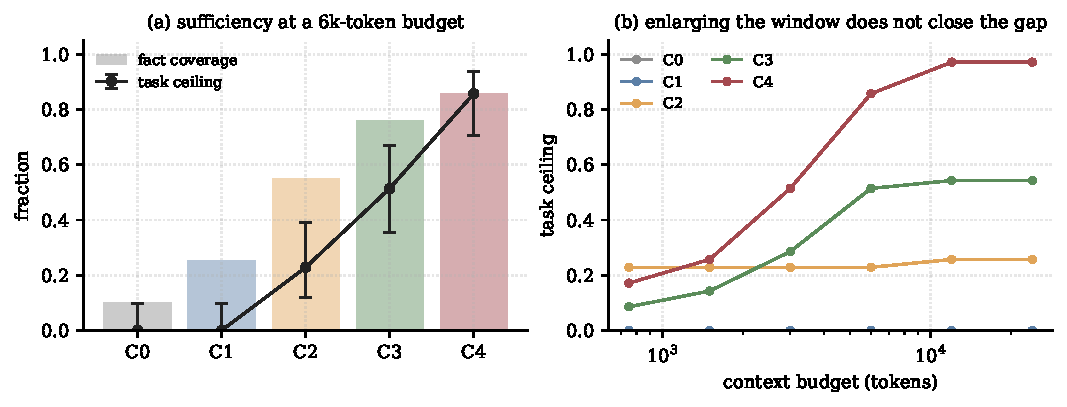
\includegraphics[width=\linewidth]{figures/fig_ceiling}
\caption{(a) Fact coverage (bars) and task ceiling (line, Wilson $95\%$
intervals) at a \TokenBudget-token budget. (b) Ceiling against context budget on
a logarithmic scale. The C2 curve is flat: a fully typed information model gains
$2.8$ percentage points as the window grows $32\times$.}
\label{fig:ceiling}
\end{figure*}

Fact coverage rises monotonically, $0.100 \to 0.252 \to 0.549 \to 0.761 \to
0.857$, but the ceiling, which requires \emph{complete} coverage, rises much
more sharply: \CeilingCZero{}, \CeilingCOne{}, \CeilingCTwo{}, \CeilingCThree{},
\CeilingCFour{}. Partial evidence is of limited value: a task with $80\%$ of its
required facts present still forces the agent to guess.

Three results merit separate discussion.

\paragraph{(i) The typed-model plateau.} Figure~\ref{fig:ceiling}b reports the
central quantitative result of the ablation. Increasing the context budget from
$750$ to $24{,}000$ tokens, a factor of $32$, moves C2's ceiling from $0.229$ to
$0.257$, and C4's from $0.171$ to $0.971$. A fully typed information model does
not become sufficient as the window grows, because the missing facts are not
located elsewhere in the document; they are \emph{absent} from it. Conversely, the
richer representations are budget-limited rather than representation-limited, so
additional context resolves their shortfall.

\paragraph{(ii) The layer responsible for each capability.}
The category columns of Table~\ref{tab:e6-ceiling} localise the effect. C2
already handles grounding ($1.00$) and most range reasoning ($0.60$). Adding
units and topology (C3) raises unit-correct reporting from $0.00$ to $0.80$ and
topology from $0.00$ to $1.00$, neither of which improves with additional type
information. Adding behaviour, constraints and provenance (C4) raises action
legality from $0.00$ to $1.00$, interlock safety from $0.00$ to $1.00$, provenance
from $0.00$ to $0.75$ and recipe conformance from $0.00$ to $1.00$. Every category
is enabled by exactly one layer, which is the non-substitutability claim of
\S\ref{sec:framework} confirmed empirically.

\paragraph{(iii) Richness competes for budget.} C4 scores $0.80$ on grounding
where C3 scores $1.00$, and $0.60$ on range reasoning where C3 scores $0.80$.
This is not noise: at a fixed budget the additional interlock, event and state
material displaces signal records that other questions require. It is a genuine
cost of semantic richness. As \S\ref{sec:e9} shows, it is a cost of serialising an
entire neighbourhood, not a property of the representation, and it is eliminated
once retrieval allocates budget to a layer only when the question requires it.

\begin{table*}[t]
\centering
\caption{E3: token bill of the identical plant in each interchange format (17 assets\, 73 signals\, 2\,465 triples).}
\label{tab:e3-serialisation}
\footnotesize
\resizebox{\ifdim\width>\linewidth\linewidth\else\width\fi}{!}{%
\begin{tabular}{lrrr}
\toprule
Serialisation & KiB & Tokens & vs.\ CSV \\
\midrule
Historian CSV (tags only) & 3.8 & 2\,256 & 1.0$\times$ \\
NGSI-LD entities (JSON-LD) & 18.4 & 11\,233 & 5.0$\times$ \\
WoT Thing Descriptions (JSON-LD) & 31.1 & 18\,471 & 8.2$\times$ \\
RDF Turtle (full KG) & 99.3 & 45\,803 & 20.3$\times$ \\
OPC UA NodeSet2 (XML) & 112.6 & 52\,324 & 23.2$\times$ \\
AAS Environment (JSON, IDTA v3) & 121.5 & 65\,929 & 29.2$\times$ \\
RDF JSON-LD (expanded) & 311.6 & 145\,216 & 64.4$\times$ \\
RDF N-Triples (full KG) & 328.2 & 179\,276 & 79.5$\times$ \\
\bottomrule
\end{tabular}}
\\[4pt]\begin{minipage}{\linewidth}\footnotesize Semantic richness is not free. An agent cannot be handed a NodeSet2 or an AAS environment directly; the graph must be \emph{queried}, and the answer, rather than the model, placed in the window.\end{minipage}
\end{table*}


\begin{figure*}[t]
\centering
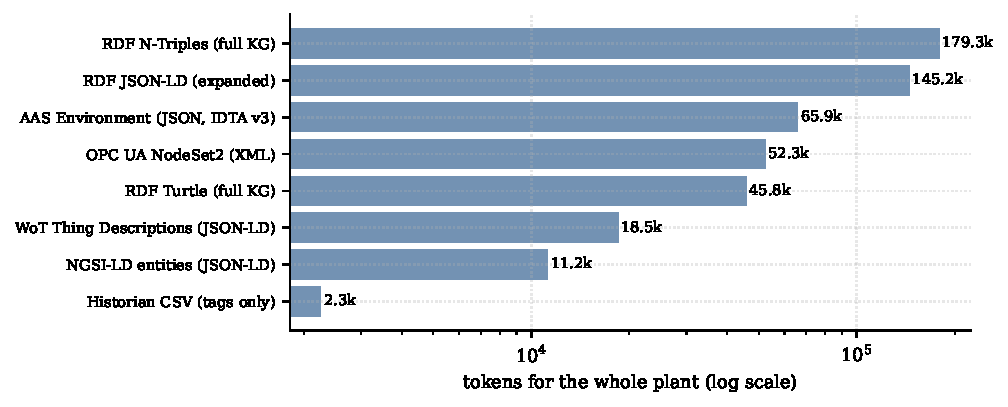
\includegraphics[width=0.86\linewidth]{figures/fig_tokens}
\caption{Token cost of the identical plant across interchange formats
(logarithmic axis). The information content is the same in every bar.}
\label{fig:tokens}
\end{figure*}

Table~\ref{tab:e3-serialisation} quantifies the token cost of semantic richness.
The same \NAssets{} assets and \NSignals{} signals cost $2{,}256$ tokens as a
historian CSV, $52{,}324$ as \opcua{} NodeSet2 ($23\times$), $65{,}929$ as an AAS
environment ($29\times$) and roughly $179{,}000$ as N-Triples
($\MaxSerialRatio\times$). Context economy, measured as coverage per thousand
tokens, is lowest at C2 ($0.106$) and recovers at C3--C4 ($0.143$, $0.162$): a
typed model is verbose without being sufficient, whereas the ontological layers
convert their verbosity into answerable questions. The practical implication is
that these formats are transfer syntaxes for machines with storage, not context
for models with bounded windows.

\subsection{E4: Guardrail efficacy}

\begin{table*}[t]
\centering
\caption{E4: guardrail efficacy over 137 proposed agent actions (84 faulty, 53 valid).}
\label{tab:e4-tiers}
\footnotesize
\resizebox{\ifdim\width>\linewidth\linewidth\else\width\fi}{!}{%
\begin{tabular}{llccccrc}
\toprule
Tier & Semantic assets available & Caught & Recall & 95\% CI & Correct diag. & False alarms & FP rate \\
\midrule
G0 & none & 0/84 & 0.000 & [0.00, 0.04] & 0.000 & 0 & 0.000 \\
G1 & JSON call schema (keys, datatypes, enumerations) & 12/84 & 0.143 & [0.08, 0.23] & 0.143 & 0 & 0.000 \\
G2 & tag dictionary, engineering ranges, unit \textbackslash{}emph{string} & 57/84 & 0.679 & [0.57, 0.77] & 0.631 & 4 & 0.075 \\
G3 & G2 + RDF/OWL graph, SHACL, QUDT dimensions and conversions, ISA-95 mereology & 62/84 & 0.738 & [0.64, 0.82] & 0.738 & 0 & 0.000 \\
G4 & G3 + PackML behaviour, explicit interlocks, SOSA/PROV observations & 84/84 & 1.000 & [0.96, 1.00] & 1.000 & 0 & 0.000 \\
\bottomrule
\end{tabular}}
\\[4pt]\begin{minipage}{\linewidth}\footnotesize \emph{Correct diagnosis} requires the validator to name the right fault family, not merely to reject. G2 rejects unit-scale errors for the wrong reason and rejects legal re-expressions of a value in a different unit.\end{minipage}
\end{table*}

\begin{table*}[t]
\centering
\caption{E4: detection by fault family.}
\label{tab:e4-families}
\footnotesize
\resizebox{\ifdim\width>\linewidth\linewidth\else\width\fi}{!}{%
\begin{tabular}{llrccccc}
\toprule
Family & Failure mode & $n$ & G0 & G1 & G2 & G3 & G4 \\
\midrule
F-ACC & write to a read-only variable & 8 & 0 & 0 & 8 & 8 & 8 \\
F-CARD & missing mandatory argument & 8 & 0 & 8 & 8 & 8 & 8 \\
F-DIM & dimensionally incompatible unit & 13 & 0 & 0 & 13 & 13 & 13 \\
F-ENUM & value outside a closed enumeration & 4 & 0 & 4 & 4 & 4 & 4 \\
F-ILK & interlock / guard condition violated & 3 & 0 & 0 & 0 & 0 & 3 \\
F-RANGE & value outside the engineering range & 8 & 0 & 0 & 8 & 8 & 8 \\
F-REF & reference to a non-existent tag or asset & 12 & 0 & 0 & 12 & 12 & 12 \\
F-SCOPE & action outside the authorised ISA-95 scope & 5 & 0 & 0 & 0 & 5 & 5 \\
F-STALE & decision based on stale evidence & 4 & 0 & 0 & 0 & 0 & 4 \\
F-STATE & illegal state transition (PackML) & 7 & 0 & 0 & 0 & 0 & 7 \\
F-UNITSCALE & correct dimension, wrong scale (silent unit error) & 4 & 0 & 0 & 4 & 4 & 4 \\
F-VALUE & numeric answer contradicting the observation & 8 & 0 & 0 & 0 & 0 & 8 \\
\bottomrule
\end{tabular}}
\\[4pt]\begin{minipage}{\linewidth}\footnotesize The last five fault families, namely interlock violation, illegal state transition, stale evidence and unfaithful read-back, are invisible to every tier that lacks an explicit behavioural, constraint or provenance model, no matter how complete its type information is.\end{minipage}
\end{table*}


\begin{figure*}[t]
\centering
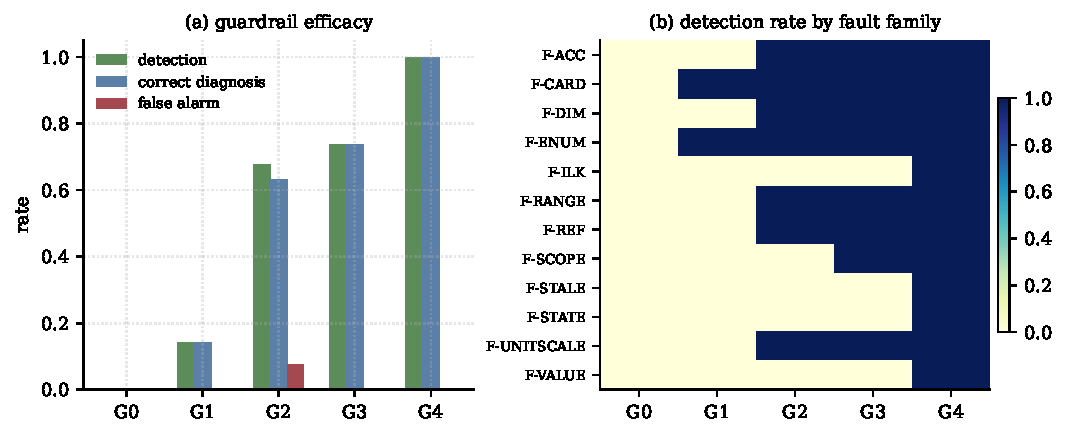
\includegraphics[width=\linewidth]{figures/fig_guardrails}
\caption{(a) Detection, correct diagnosis and false-alarm rates by validator
tier. (b) Per-family detection rate; the block structure shows each tier opening
a distinct band of fault families rather than uniformly improving.}
\label{fig:guardrails}
\end{figure*}

Over \NCases{} proposed actions (\NFaulty{} faulty), detection recall runs
\RecallGZero{}, \RecallGOne{}, \RecallGTwo{}, \RecallGThree{},
\RecallGFour{}. Three findings.

\paragraph{Limitations of the flat catalogue.} Tier~G2, a tag dictionary with
engineering ranges and a unit string, which is what most industrial ``semantic
layer'' products implement, reaches \RecallGTwo{} recall, which appears adequate.
It is, however, the only tier that raises false alarms (\FPRGTwo{} of valid
actions rejected), and its diagnosis rate ($0.631$) falls below its detection
rate: it rejects the four unit-scale errors for the wrong reason (reporting a unit
mismatch rather than a range violation) and rejects four legal actions whose only
deviation is being expressed in a different but commensurable unit. Both
behaviours share a single cause, the comparison of units as strings, and both are
detrimental in production, because an operator who observes the assistant refuse a
legal instruction loses trust faster than one who observes it make a detectable
error.

\paragraph{Each tier opens a distinct band.} Figure~\ref{fig:guardrails}b shows
the block structure plainly. G1 catches only \textsc{f-card} and \textsc{f-enum}.
G2 adds \textsc{f-ref}, \textsc{f-acc} and \textsc{f-range}. G3 adds
\textsc{f-scope} and detects \textsc{f-dim}/\textsc{f-unitscale} correctly rather
than incidentally. G4, and only G4, catches \textsc{f-ilk}, \textsc{f-state},
\textsc{f-stale} and \textsc{f-value}: twenty-two cases, $26\%$ of the faulty
corpus, comprising every failure mode that can move a plant into an unsafe or
non-conforming state. In this benchmark no tier lacking an explicit behavioural,
constraint or provenance model reaches them, however complete its type
information.

\paragraph{Full semantics does not over-constrain.} G4 attains
\RecallGFour{} recall at \FPRGFour{} false alarms and $1.000$ diagnosis. The
common objection that formal validation blocks legitimate work is not supported:
the \emph{weak} validator is the one that over-blocks, because it must be
conservative about what it cannot interpret.

\subsection{E4b: Is the gain from semantics or from any strong rule system?}

\begin{table}[t]
\centering
\caption{E4b: is the guardrail gain from \emph{any} strong rule system, or from explicit semantics? A non-RDF procedural validator (G-proc) with a hard-coded unit-conversion table is compared against the flat catalogue and the two graph tiers.}
\label{tab:e4b-procedural}
\footnotesize
\resizebox{\ifdim\width>\linewidth\linewidth\else\width\fi}{!}{%
\begin{tabular}{lcccccc}
\toprule
Validator & Recall & False alarms & FP rate & Diagnosis & Unit-scale diag. & Behavioural \\
\midrule
G2 flat catalogue (unit \emph{string}) & 0.679 & 4 & 0.075 & 0.631 & 0/4 & 0/22 \\
G-proc bespoke code (unit \emph{calculus}) & 0.679 & 0 & 0.000 & 0.679 & 4/4 & 0/22 \\
G3 RDF + SHACL + QUDT & 0.738 & 0 & 0.000 & 0.738 & 4/4 & 0/22 \\
G4 full semantic stack & 1.000 & 0 & 0.000 & 1.000 & 4/4 & 22/22 \\
\bottomrule
\end{tabular}}
\\[4pt]\begin{minipage}{\linewidth}\footnotesize \emph{Unit-scale diag.} is \emph{correct diagnosis} of \textsc{f-unitscale} (silent scale errors): the flat catalogue rejects them for the wrong reason (a unit-string mismatch), so it scores zero here although it happens to reject. \emph{Behavioural} is detection across \textsc{f-ilk}, \textsc{f-state}, \textsc{f-stale} and \textsc{f-value}. Procedural code with a unit calculus matches the RDF+QUDT tier on the unit families and eliminates the flat catalogue's false alarms, so the unit result is \emph{not} RDF-specific. The behavioural, interlock, temporal and provenance families remain out of reach until the corresponding model is re-implemented by hand; the semantic stack supplies each as a declarative, reusable asset instead.\end{minipage}
\end{table}


A natural objection is that G4's advantage reflects having \emph{any} sufficiently
strong rule engine, not the semantic stack in particular. Experiment~E4b tests it
directly (Table~\ref{tab:e4b-procedural}) with a non-RDF procedural validator,
G-proc: the checks a competent engineer would hand-write on a typed catalogue
augmented with a hard-coded unit-conversion table, with no RDF graph, no SHACL, no
interlock or state model and no provenance store. The result splits cleanly along
exactly the line the paper draws. On \emph{units}, G-proc matches the RDF+QUDT
tier: it removes all \GTwoFalseAlarms{} of the flat catalogue's false alarms and
correctly diagnoses every silent scale error, so the unit result is a property of
having a \emph{calculus}, not of RDF, and we do not claim otherwise. On
\emph{behaviour} G-proc collapses to the flat catalogue, catching
\ProcBehavCaught{} of the \ProcBehavN{} interlock, illegal-state, staleness and
faithfulness faults: these require the interlock model, the PackML state machine
and the observation store, none of which a unit table holds. The distinctive
contribution of the semantic stack is thus the behavioural, constraint and
provenance models, supplied as declarative and reusable assets; bespoke code can
reach the same faults only by re-implementing each model by hand, per plant, and
maintaining and testing it there, which is the cost the semantic approach removes.

\subsection{E5: The admissible action space}

\begin{table*}[t]
\centering
\caption{E5: size and fidelity of the admissible action space.}
\label{tab:e5-actionspace}
\footnotesize
\resizebox{\ifdim\width>\linewidth\linewidth\else\width\fi}{!}{%
\begin{tabular}{lrrcc rrcc}
\toprule
Tier & $|A|$ & $\Delta$bits & Prec. & Rec. & $|A|$ & $\Delta$bits & Prec. & Rec. \\
\midrule
G0 & 71\,540 & 0.00 & 0.010 & 1.000 & 153 & 0.00 & 0.170 & 1.000 \\
G1 & 71\,540 & 0.00 & 0.010 & 1.000 & 153 & 0.00 & 0.170 & 1.000 \\
G2 & 190 & 8.56 & 0.937 & 0.251 & 81 & 0.92 & 0.321 & 1.000 \\
G3 & 755 & 6.57 & 0.940 & 1.000 & 81 & 0.92 & 0.321 & 1.000 \\
G4 & 710 & 6.65 & 1.000 & 1.000 & 26 & 2.56 & 1.000 & 1.000 \\
\bottomrule
\end{tabular}}
\\[4pt]\begin{minipage}{\linewidth}\footnotesize Left block: \texttt{write\_setpoint(tag,value,unit)} enumerated over $73$ tags $\times$ $35$ units $\times$ $28$ magnitudes. Right block: \texttt{packml\_command(asset,command)}. \emph{Precision} is the probability that an admitted call is genuinely executable; \emph{recall} is the fraction of executable calls the tier still allows. G2 buys its reduction by forbidding legal work.\end{minipage}
\end{table*}

\begin{table}[t]
\centering
\caption{E5: size of the generated \texttt{write\_setpoint} tool schema for Line 1.}
\label{tab:e5-schema}
\footnotesize
\resizebox{\ifdim\width>\linewidth\linewidth\else\width\fi}{!}{%
\begin{tabular}{lr}
\toprule
Cond. & Schema tokens \\
\midrule
C0 & 205 \\
C1 & 218 \\
C2 & 981 \\
C3 & 1\,669 \\
C4 & 2\,317 \\
\bottomrule
\end{tabular}}
\\[4pt]\begin{minipage}{\linewidth}\footnotesize Constraints carried in the schema are enforced by constrained decoding; constraints left out must be recalled by the model.\end{minipage}
\end{table}


\begin{figure*}[t]
\centering
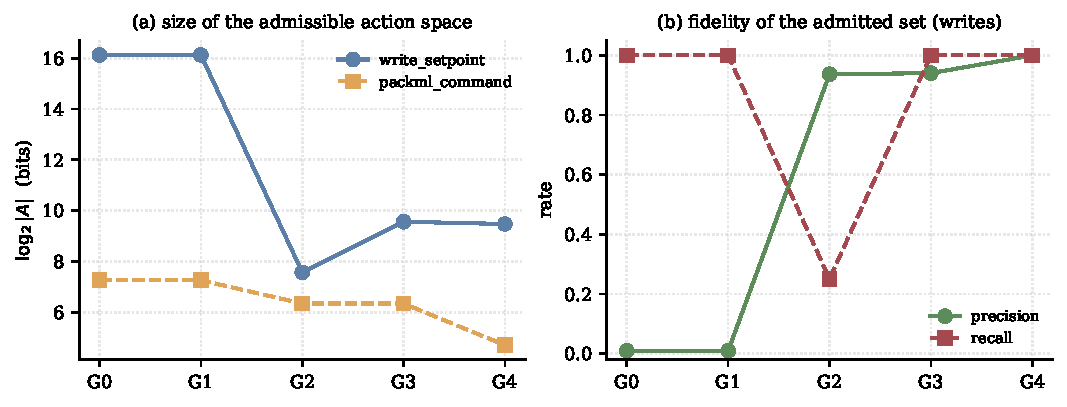
\includegraphics[width=\linewidth]{figures/fig_actionspace}
\caption{(a) Size of the admissible action space in bits. (b) Precision and
recall of the admitted set for \texttt{write\_setpoint}. G2 achieves its
reduction partly by excluding legal actions.}
\label{fig:actionspace}
\end{figure*}

Enumerating $\NSignals{} \times 35 \times 28 = 71{,}540$ syntactically
well-formed \texttt{write\_setpoint} calls, only $710$ are genuinely executable
which gives a prior probability of \ActPrecGZero{} that an arbitrary well-formed call is
legal. This quantifies the risk of unconstrained tool use in an OT environment.

Tier~G2 removes $8.56$ bits, admitting $190$ calls at \ActPrecGTwo{} precision
but only at \ActRecGTwo{} recall. It forbids three quarters of the legal action
space, all of it consisting of values correctly expressed in a commensurable
unit. Tier~G3 admits $755$ calls at $0.940$ precision and full recall; tier~G4
admits $710$ at \ActPrecGFour{} precision and \ActRecGFour{} recall, the
difference being the two tags whose interlocks are currently unsatisfied. For
PackML commands the effect is larger: of $153$ well-formed calls, $26$ are legal,
so a tier without the state machine offers at best $0.321$ precision whereas G4
reaches $1.000$.

Table~\ref{tab:e5-schema} shows the cost of pushing these constraints into the
tool schema itself: $205$ tokens for an unconstrained
\texttt{write\_setpoint}, $2{,}317$ for the fully constrained version carrying
tag enumerations, per-tag ranges, accepted units, semantic identifiers, interlock
status and the current legal command set. Two thousand tokens is a modest cost
for moving $6.65$ bits of constraint from the model's memory into the decoder's
grammar; moreover, a tool schema is paid once per session rather than once per
turn.

\subsection{E7: Query execution versus context stuffing}

\begin{table*}[t]
\centering
\caption{E7: answering by query execution instead of context stuffing.}
\label{tab:e7-sparql}
\footnotesize
\resizebox{\ifdim\width>\linewidth\linewidth\else\width\fi}{!}{%
\begin{tabular}{llrrrrrcr}
\toprule
Task & SPARQL probe & Query & Rows & Result & Total & C4 tok. & Suff.? & Saving \\
\midrule
UNI-05 & Total electrical power drawn by the utilities area, unit-normalised & 152 & 1 & 1 & 153 & 5\,373 & \checkmark & 35.1$\times$ \\
RNG-04 & Every tag in the plant whose latest observation violates an alarm limit & 197 & 1 & 25 & 222 & 741 & $\times$ & 3.3$\times$ \\
TOP-02 & Transitive downstream closure of the Line 1 pasteuriser & 56 & 3 & 23 & 79 & 5\,461 & \checkmark & 69.1$\times$ \\
TOP-03 & Every asset belonging to Bottling Line 1 & 62 & 5 & 77 & 139 & 5\,172 & \checkmark & 37.2$\times$ \\
ACT-04 & Line 1 units that accept Start in their current PackML state & 76 & 1 & 8 & 84 & 5\,172 & \checkmark & 61.6$\times$ \\
SAF-04 & Writable Line 1 tags protected by an interlock & 101 & 3 & 140 & 241 & 5\,172 & \checkmark & 21.5$\times$ \\
PRV-04 & Alarms upstream of the Line 1 capper in the preceding five minutes & 172 & 3 & 115 & 287 & 5\,492 & \checkmark & 19.1$\times$ \\
GRD-01 & Grounded lookup of one homograph-laden mention & 130 & 1 & 19 & 149 & 5\,501 & \checkmark & 36.9$\times$ \\
\bottomrule
\end{tabular}}
\\[4pt]\begin{minipage}{\linewidth}\footnotesize All queries execute against the same RDF graph and return the correct answer. \emph{Suff.?} records whether the stuffed C4 context contained every required fact. RNG-04 is a plant-wide sweep: it is unanswerable by stuffing at any budget, yet costs 222 tokens as a query.\end{minipage}
\end{table*}


Eight questions answered two ways. Stuffed C4 contexts cost $5{,}172$--$5{,}501$
tokens; the same questions answered by SPARQL cost $79$--$314$ tokens including
the query text, a saving of $17.5$ to $\MaxQuerySaving\times$. Every query
returns the correct answer.

The clearest case is RNG-04, ``which tags anywhere in the plant are outside their
alarm limits''. Its evidence is every observation and every alarm limit in the
plant; no top-$k$ retrieval assembles it, and the sweep confirms the stuffed
context is insufficient at every budget tested. As a query it costs $222$ tokens
and returns one row. A class of industrial questions, aggregate, plant-wide and
threshold-crossing, is not a context-assembly problem at all; under top-$k$
retrieval at every budget tested, treating it as one yields an incorrect answer.

\subsection{E8: Is grounding robust to the naming convention?}
\label{sec:e8}

\begin{table*}[t]
\centering
\caption{E8: grounding under five tag naming conventions. Descriptions, relations, units, ranges, states and values are identical in every row; only the identifier strings differ. Cells are top-1 accuracy with the fraction resolved \emph{confidently to the wrong tag} in parentheses.}
\label{tab:e8-convention}
\footnotesize
\resizebox{\ifdim\width>\linewidth\linewidth\else\width\fi}{!}{%
\begin{tabular}{llcccc}
\toprule
Naming scheme & Example & C1 & C1+conv & C2+conv & C4 \\
\midrule
ISA-5.1 mnemonic (baseline) & \texttt{L1\_FIL\_PT0301\_PV} & 0.79\,(0.21) & 0.95\,(0.05) & 0.95\,(0.05) & 1.00\,(0.00) \\
sequential I/O address & \texttt{AI\_04213} & 0.53\,(0.47) & 0.53\,(0.47) & 0.95\,(0.05) & 1.00\,(0.00) \\
KKS / RDS-PP designation & \texttt{=1LCA10CP001XQ01} & 0.89\,(0.11) & 0.89\,(0.11) & 0.95\,(0.05) & 1.00\,(0.00) \\
OEM browse path & \texttt{Krones.Modulfill.Ch17.Value} & 0.42\,(0.58) & 0.42\,(0.58) & 0.95\,(0.05) & 1.00\,(0.00) \\
mnemonic, but misleading & \texttt{L2\_PAS\_PT0301\_PV} & 0.84\,(0.16) & 0.63\,(0.37) & 0.95\,(0.05) & 1.00\,(0.00) \\
\midrule
\emph{spread across conventions} &  & \textbf{0.47} & \textbf{0.53} & \textbf{0.00} & \textbf{0.00} \\
\bottomrule
\end{tabular}}
\\[4pt]\begin{minipage}{\linewidth}\footnotesize \textbf{C1} = description text only. \textbf{C1+conv} = description $+$ decoded mnemonic. \textbf{C2+conv} = typed model $+$ decoded mnemonic. \textbf{C4} = resolve the asset, then search its scope. Decoding the mnemonic is the strongest available reading of an un-grounded catalogue, and on the convention it was built for it nearly matches a typed model. It is also the only resolver whose accuracy \emph{falls} when the convention stops being truthful, and the only one whose accuracy varies with the convention at all.\end{minipage}
\end{table*}


Experiment~E1 showed a plain historian export resolving \GrndTopOneCOne{} of
mentions. That figure explains why un-grounded pipelines perform well in
demonstrations, and it warrants scrutiny, because it rests on something no machine
has verified: the tag mnemonic. \texttt{L1\_FIL\_PT0301\_PV} indicates, to a
reader who knows the convention, a pressure transmitter on the Line~1 filler. This
is genuine semantics, but it is unwritten, unversioned, unenforced and
site-specific.

E8 re-tags the plant under \NSchemes{} conventions drawn from real installations
including ISA-5.1 mnemonics, sequential I/O addresses, KKS designations, OEM browse
paths, and a post-merger plant whose mnemonics survive but no longer describe
the asset they are attached to. Descriptions, relations, units, ranges, states
and values are identical throughout; only identifier strings move.

The baseline is deliberately \emph{strengthened} for this test. Resolver
\texttt{C1+conv} is permitted to decode the mnemonic, expanding \texttt{FIL}
to ``filler'', \texttt{PT} to ``pressure'', \texttt{L1} to ``line 1'', which
is exactly what a language model does when handed a tag list, and which a
bag-of-words retriever does not do. Three results follow.

\paragraph{On the convention it was built for, decoding nearly matches a typed
model.} \texttt{C1+conv} reaches \ConvMnemonicDecoded{} on the mnemonic scheme,
against $95\%$ for the typed model. An organisation measuring only this
configuration would reasonably conclude that its tag catalogue is sufficient.

\paragraph{The capability does not survive a change of convention.} Accuracy
varies from \ConvWorstCOnePlusconv{} to \ConvBestCOnePlusconv{} across the five
schemes, a spread of \ConvSpreadCOnePlusconv{} percentage points. On sequential
I/O addresses and OEM browse paths there is nothing to decode, and the resolver
collapses back to description matching. The typed model and the graph vary by
\ConvSpreadCTwoPlusconv{} and \ConvSpreadCFour{} points respectively: they are
\emph{invariant}, because membership is stated rather than inferred.

\paragraph{When the convention is untruthful, decoding underperforms ignoring it.}
On the inconsistent plant, \texttt{C1+conv} scores \ConvLyingDecoded{}, below the
$0.84$ of the same resolver with decoding switched off, and resolves
\ConvLyingWrong{} of mentions confidently to the wrong tag. The convention is
syntactically perfect and semantically false, and nothing in the representation
contradicts it. This illustrates precisely what ``ungrounded'' means: not that the
system is uninformed, but that it cannot be corrected.

Two further observations. First, convention-invariance is bought at C2, not C3
because an explicit membership relation is enough; the ontology is not required for
\emph{this} property. Second, the graph resolver is the only one that never
answers confidently and wrongly ($0.00$ in every row), because a mention it
cannot resolve to an asset yields nothing rather than a plausible neighbour.

\subsection{E9: Intent-routed projection}
\label{sec:e9}

\begin{table*}[t]
\centering
\caption{E9: neighbourhood projection versus intent-routed projection at a 6000-token budget.}
\label{tab:e9-routing}
\footnotesize
\resizebox{\ifdim\width>\linewidth\linewidth\else\width\fi}{!}{%
\begin{tabular}{ll ccc cccccccc}
\toprule
Cond. & Projection & Ceiling & Coverage & Verif@1 & GRD & UNI & RNG & TOP & PRV & ACT & SAF & REC \\
\midrule
C3 & neighbourhood & 0.514 & 0.761 & 1.000 & 1.00 & 0.80 & 0.80 & 1.00 & 0.00 & 0.00 & 0.00 & 0.00 \\
C3 & routed & 0.543 & 0.774 & 1.000 & 1.00 & 1.00 & 0.80 & 1.00 & 0.00 & 0.00 & 0.00 & 0.00 \\
C4 & neighbourhood & 0.857 & 0.857 & 0.842 & 0.80 & 0.80 & 0.60 & 1.00 & 0.75 & 1.00 & 1.00 & 1.00 \\
C4 & routed & 0.943 & 0.959 & 1.000 & 1.00 & 0.80 & 0.80 & 1.00 & 1.00 & 1.00 & 1.00 & 1.00 \\
\bottomrule
\end{tabular}}
\\[4pt]\begin{minipage}{\linewidth}\footnotesize Routing spends budget on the constraint, event and recipe layers only when the question gives a reason to, using surface cues available before retrieval. No category degrades; grounding and provenance recover fully. The trade-off between semantic richness and context budget is therefore an artefact of dumping a neighbourhood, not a property of the representation.\end{minipage}
\end{table*}


\begin{figure*}[t]
\centering
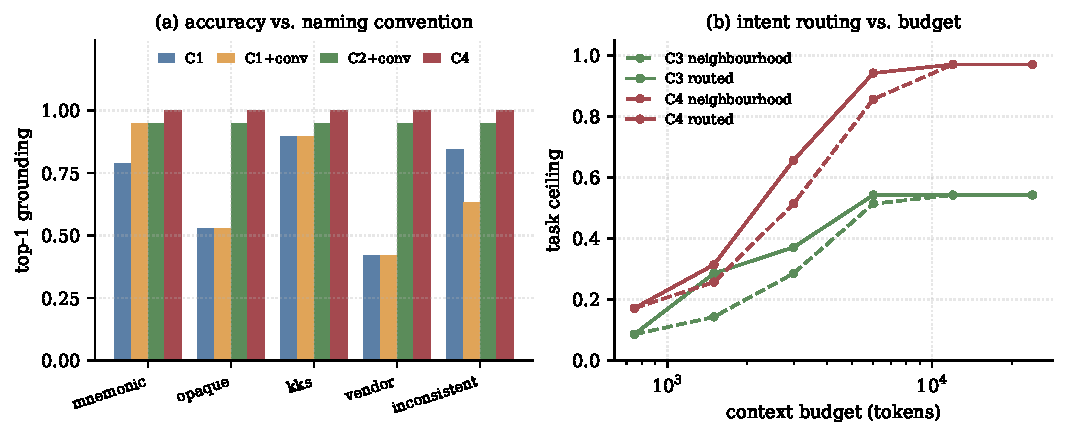
\includegraphics[width=\linewidth]{figures/fig_convention}
\caption{(a) E8: top-1 grounding under five naming conventions. Only the
resolvers that read an explicit membership relation are flat. (b) E9: task
ceiling against budget for neighbourhood projection (dashed) and intent-routed
projection (solid).}
\label{fig:convention}
\end{figure*}

The richness-versus-budget effect of \S\ref{sec:results}(iii) is a property of
\emph{how} the graph neighbourhood is serialised, not of what it contains. A
question such as ``what is the bowl level of the Line 1 filler?'' gives no
reason to spend budget on interlocks, event logs or recipe parameters, yet the
neighbourhood projector fetches them because they are topologically close.

Intent routing uses surface cues available \emph{before} retrieval, modal and
imperative verbs for behaviour, temporal and causal words for provenance,
specification words for recipes, to decide which layers to fetch ahead of
payload. The lexicon is small and inspectable; the claim is not that it is
optimal but that the signal is cheap.

The trade-off is eliminated. At the \TokenBudget-token budget the C4 ceiling rises
from \RouteCFourNeighCeiling{} to \RouteCFourRoutedCeiling{}, and verifiable
grounding from \RouteCFourNeighVerif{} to \RouteCFourRoutedVerif{}, at
essentially identical cost (\RouteCFourNeighTokens{} against
\RouteCFourRoutedTokens{} tokens). No category degrades: grounding returns to
$1.00$, provenance from $0.75$ to $1.00$, range reasoning from $0.60$ to
$0.80$, while action legality and interlock safety remain at $1.00$.
Figure~\ref{fig:convention}b shows that the gain is largest where the budget is
tightest: C4 at $3{,}000$ tokens rises from $0.514$ to $0.629$. This is the
operationally relevant regime, since a deployed agent shares its window with
instructions, tool schemas and history.

The conclusion is not that richness is free, but that it is costly only when
projected indiscriminately. A representation with several content layers and no
mechanism for selecting the one the question requires expends its budget on the
others.

\subsection{E11: A real-model sanity check}
\label{sec:e11}

\begin{table}[t]
\centering
\caption{E11: real-model sanity check. Model \texttt{gpt-5.6-sol}, 3 repeats, 35 tasks per condition, accessed 2026-10-06. A dated measurement; unlike every other table it is not regenerated by the deterministic pipeline.}
\label{tab:e11-realmodel}
\footnotesize
\resizebox{\ifdim\width>\linewidth\linewidth\else\width\fi}{!}{%
\begin{tabular}{lccccc}
\toprule
Cond. & Accuracy & Ceiling & Refusal & Halluc.(ins.) & Acc.$|$suff \\
\midrule
C0 & 0.00 & 0.00 & 1.00 & 0.00 & -- \\
C1 & 0.14 & 0.00 & 0.85 & 0.01 & -- \\
C2 & 0.29 & 0.23 & 0.63 & 0.10 & 0.96 \\
C3 & 0.40 & 0.51 & 0.51 & 0.00 & 0.78 \\
C4 & 0.55 & 0.86 & 0.28 & 0.00 & 0.64 \\
\bottomrule
\end{tabular}}
\\[4pt]\begin{minipage}{\linewidth}\footnotesize \emph{Accuracy} is graded heuristically against the gold answers (raw answers are archived for audit). \emph{Ceiling} is the model-free sufficiency bound (Table~\ref{tab:e6-ceiling}); \emph{Halluc.(ins.)} is the fraction of insufficient-context tasks answered wrongly rather than refused; \emph{Acc.$|$suff} is accuracy on sufficient-context tasks. Accuracy rises monotonically with the stack; it exceeds the ceiling at C1--C2, where the model guesses from naming conventions (\S\ref{sec:e8}), and falls below it at C3--C4, the model-execution gap the ceiling bounds.\end{minipage}
\end{table}


The results above are model-free by construction. To check that the ceilings
predict the behaviour of a real agent, we ran the task suite through a
contemporary model (\texttt{\EllModel}, \EllRepeats{} repeats per task, accessed
\EllDate) using the adapter of \S\ref{sec:llm-adapter}. This is a dated sanity
check rather than a contribution: a single model's scores would age and do not
bear on the representational claims. We include it because a reviewer reasonably
asks whether representation ceilings track real success.

\begin{figure*}[t]
\centering
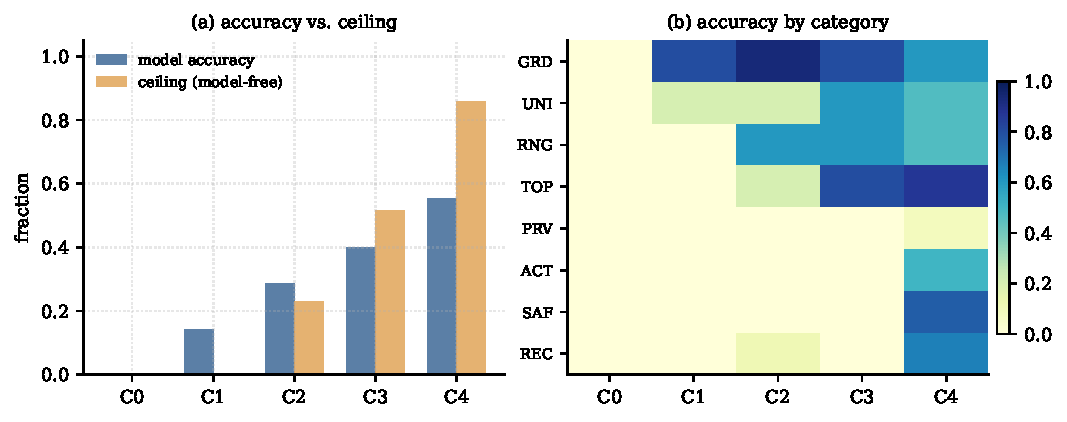
\includegraphics[width=\linewidth]{figures/fig_e11}
\caption{E11. (a) Real-model accuracy against the model-free sufficiency ceiling
by condition. (b) Per-category accuracy by condition; the block structure
reproduces the ceiling's (Table~\ref{tab:e6-ceiling}).}
\label{fig:e11}
\end{figure*}

Three things hold, and all three were predicted. \textbf{First}, accuracy rises
monotonically with the semantic stack, \EllAccCZero{} $\to$ \EllAccCOne{} $\to$
\EllAccCTwo{} $\to$ \EllAccCThree{} $\to$ \EllAccCFour{}, and the per-category
pattern matches the ceiling almost exactly (Figure~\ref{fig:e11}b): action
legality, interlock safety, recipe conformance and provenance remain at zero until
C4 supplies the behavioural, constraint and provenance layers, while topology and
unit reporting appear at C3. The layer that unlocks a category for an ideal reader
is the layer that unlocks it for this model.

\textbf{Second}, where evidence is sufficient the model stays \emph{below} the
ceiling, by a margin that widens with task difficulty: accuracy on
sufficient-context tasks falls from $0.96$ at C2 to $0.64$ at C4, because the
tasks C4 makes answerable are the multi-step behavioural and safety questions. The
ceiling is an upper bound, as stated in \S\ref{sec:threats}, and a real model does
not saturate it.

\textbf{Third}, at C1 and C2 accuracy \emph{exceeds} the ceiling (\EllAccCOne{}
against a $0\%$ ceiling, \EllAccCTwo{} against $23\%$). This is not a
contradiction but the unverifiable competence of \S\ref{sec:e8} appearing on cue:
with no stated membership facts the model answers correctly by decoding tag
mnemonics, the capability E8 shows is non-transferable and collapses when the
convention changes or is untruthful. The excess accuracy is exactly the part that
cannot be audited. Both halves of the construct-validity caveat of
\S\ref{sec:threats} are thus observed in one run: the model guesses above the
ceiling where conventions permit, and falls below it where reasoning is hard.

Refusal behaviour supports this reading. Instructed to answer only from the
context, the model produced a wrong, non-refused answer on at most $10\%$ of
insufficient-context tasks (C2) and none at C3--C4: it fails safe far more often
than it fails loud. We stress the limits of this check: one model, one date, a
heuristic grader with the raw answers archived for audit, and \EllRepeats{}
repeats; it corroborates the ordering, and nothing more is claimed of it.

\subsection{Summary of results}

\begin{table*}[t]
\centering
\caption{Headline effects. Each row is a capability, the layer that supplies it,
and the measured consequence of its absence.}
\label{tab:headline}
\footnotesize
\setlength{\tabcolsep}{4pt}
\begin{tabular}{@{}L{3.6cm}L{2.6cm}L{9.0cm}@{}}
\toprule
\textbf{Capability} & \textbf{Layer} & \textbf{Measured effect of adding it} \\
\midrule
Descriptions \& identity & L0/L1 & grounding \GrndTopOneCZero{} $\to$
\GrndTopOneCOne{} top-1 \\
Types, ranges, access & L1 & grounding $\to$ \GrndTopOneCTwo{}; guardrail recall
$\to$ \RecallGTwo{}; ceiling $\to$ \CeilingCTwo{} \\
Unit calculus & L3 (QUDT) & unit-correct reporting $0.00 \to 0.80$; removes all
\FPRGTwo{} false alarms; action recall \ActRecGTwo{} $\to$ \ActRecGThree{} \\
Topology \& mereology & L2/L1 & topology tasks $0.00 \to 1.00$; enables
\textsc{f-scope} detection \\
Behavioural model & L1 (PackML/MTP) & action-legality tasks $0.00 \to 1.00$;
command-space precision $0.321 \to 1.000$ \\
Explicit constraints & L2 (SHACL) & interlock tasks $0.00 \to 1.00$; guardrail
recall $\to$ \RecallGFour{} \\
Provenance \& observations & L3 (SOSA/PROV) & provenance tasks $0.00 \to 0.75$;
makes answer faithfulness checkable \\
Query pushdown & L2 (SPARQL) & up to $\MaxQuerySaving\times$ token saving;
answers questions no window holds \\
\bottomrule
\end{tabular}
\end{table*}
